Partial differential equations (PDE's) are ubiquitous among the tools for modeling complex phenomena in all sciences. However, we almost never have explicit solutions for them, making it difficult to describe those phenomenons and make accurate predictions about them. Hence, we need numerical methods to provide approximate solutions to those equations, for example, classical methods are finite differences, finite elements and spectral methods. Those rely on different discretizations of the particular problem that  we can use for calculating approximations in different forms and with varying levels of accuracy. Since the advent of fast computers and efficient tools for programming them, this process is effective for many kinds of problems.   

Now, when we attempt to solve numerically some particular problem, we need to play with the trade-off between accuracy of the approximate solution and the computational cost needed to obtain it. Indeed, with those classical methods, a small approximation error requires a finer grid, which implies more computational resources to store and process the information required by the method. In consequence, for some problems, we may not be able to calculate an accurate enough solution in a feasible computational time.

This is the case for high dimensional PDE's, for which the size of discretization usually scales exponentially with the number of points used for each dimension. For example, if we try to use a finite difference scheme in a $100$-dimensional unit square $[0,1]^{100}$ with $N$ points in each dimension, we would need $N^{100}$ points in total, making it impossible to even store them in a computer. In practice, high dimension can be considered as low as $d>4$, for which traditional methods cannot be used as regularly. This problem is known as the \textit{curse of dimensionality}, a term established by Bellman when considering problems in dynamic programming.

High dimensional PDE's appear in many contexts, such as asset pricing, image denoising, statistical physics, many-body quantum mechanics, optimal control and game theory. Therefore, there is a necessity for numerical methods that are able to overcome this difficulty. Early attempts to solve this kind of problems used the connection between stochastic diffusions and parabolic PDE's, as we seemed in the preceding chapter. In fact, if the PDE is linear, the linear Feynman-Kac \ref{thm:LinearFK} formula can be used to provide an approximate solution by computing the expectation using simulated paths of the process through the  Monte-Carlo approach. The convergence of this formulation is \hlc[Sure?]{independent} of the dimension of the underlying process, and therefore does not suffer from the curse dimensionality.

Nevertheless, if we try a similar approach using the non-linear Feynman-Kac formula \ref{thm:NonlinealFK} for more general non-linear equations, we would have to deal with solving numerically the associated BSDE. There are numerical methods to approximate the set of solution processes $(X,Y,Z)$, but they are not as simple as an Euler-Maruyama discretization for a forward process. Generally, they require the computation of conditional expectations that almost never are computationally cheap and hence is not a straightforward generalization of the former linear approach. Despite this, some progress has been made under this formulation, see for example \cite{chessari_numerical_nodate}. Other solutions methods are based in fixed point iterations and branching methods \cite{bibid}.

Representing functions in a high dimensional space is a problem encountered in many other areas of applied mathematics. Particularly, in recent times, the analysis and inference on big amounts of data has emerged as the fascinating research area of \textit{machine learning}. Many methods have been proposed for this goal, for example, regression methods, support vector machines and tree methods. Nonetheless, the approach that has encountered more success when trying to approximate high dimensional functions using big amounts of data is deep learning.  In this setting, we parametrize functions using structures that use composition of simpler function for approximate complex ones, these structures are called neural networks. We refer the reader to \autoref{chp:ApendixNN} for a brief introduction and to \cite{higham_deep_2019} for a deeper exposition of the topic.

The idea of using this neural network parametrization of functions to solve PDE's can be tracked to the 80's, when in \cite{} a perceptron layer approximation was proposed to \hlc[Completar]{}. However, due to the high computational cost of training a neural network, a successful attempt was not achieved until recently, with the works of \cite{bibid}\hlc[Blablabla]{}. 

This is a very new area of research, for which many open questions remain. Particularly, it is not well understood yet if the curse of dimensionality is solved, even if there is work for certain equations that ensures it \cite{bibid}. Also, there is not yet a good understanding of why different classes of neural networks are useful to approximate certain classes of functions and how to tune adequately its parameters to do it efficiently. In consequence, even if it is possible to give a convergence proof for certain cases, most algorithms rely on empirical experimentation and heuristic arguments to provide reasonable approximate solutions.    

In this chapter we review some of these methods, implement them for toy examples and perform a comparison of speed, accuracy and practical usefulness for solving PDE's.   

\section{Free boundary problems}
Let's start with problems in free space. In the same setup as \autoref{thm:verficationThm}, we deal with the following equation with terminal condition
\begin{equation}
	\label{eqn:FKNolinealCh2}
	\begin{split}
		&\dpartial{v}{t}(t,x)+\mu(t,x)\cdot D_x v(t,x)+\frac{1}{2}\Tr(\sigma(t,x)\sigma^{T}(t,x)D_{xx}^2v(t,x))\\
		&+f(t,x,v(t,x),\sigma(t,x)' D_x v(t,x))=0\\
		&v(T,x)=g(x).
	\end{split}
\end{equation}
We have proven that we can construct a viscosity solution to this equation by setting $v(t,x)=Y_{t}^{t,x}$, where $Y$ is the solution process to the FBSDE
\begin{equation}
	\label{eqn:UncoupledCh2}
	\begin{split}
		&dX_s=\mu(s,X_s)ds+\sigma(s,X_s)dW_s\\
		&X_t=x,\\
		&dY_s=-f(s,X_s,Y_s,Z_s)ds+Z_s dW_s\\
		&Y_T=g(X_T).
	\end{split}
\end{equation}
Moreover, we have that $Y_t=v(t,X_t)$ and $Z_t=\sigma(t,X_t)'D_x v(t,X_t)$.
\subsection{Deep BSDE method}
The first deep learning algorithm that was successfully applied to solve equation \eqref{eqn:FKNolinealCh2} was proposed by Han, E and Jentzen \cite{han_solving_2018,e_deep_2017}. This algorithm aims to approximate $Y_0=v(0,x)$ for some point $x\in \bbR^n$, and is similar in spirit to the stochastic shooting method for ODE's.

Here we discretize the time domain $0=t_0<t_1<\cdots <t_{N-1}<t_N=T$ and the FBSDE system a  forward equation using the Euler-Maruyama scheme for $n=0,\ldots,N-1$,
\begin{equation}
	\label{eqn:EMForward}
	X_{t_{n+1}} \approx X_{t_n} +\mu\left(t_n, X_{t_n}\right) \Delta t_n+\sigma\left(t_n, X_{t_n}\right) \Delta W_n
\end{equation}
and 
\begin{equation}
	\label{eqn:EMBackward}
	\begin{aligned}
		 v\left(t_{n+1}, X_{t_{n+1}}\right)
		&\approx  v\left(t_n, X_{t_n}\right) -f\left(t_n, X_{t_n}, v\left(t_n, X_{t_n}\right), \sigma'\left(t_n, X_{t_n}\right) D_x v\left(t_n, X_{t_n}\right)\right) \Delta t_n \\
		& +\sigma\left(t_n, X_{t_n}\right)'D_x u\left(t_n, X_{t_n}\right)  \Delta W_n,
	\end{aligned}
\end{equation}
where $\Delta t_n=t_{n+1}-t_{n}$ and $\Delta W_n\sim \mathcal{N}(0,\Delta t_n)$.

The main idea of this algorithm is to transform the problem in a learning one approximating the unknown product $\sigma\left(t_n, X_{t_n}\right)'D_x u\left(t_n, X_{t_n}\right)$ with a fully coupled neural network for each time step, i.e
\begin{equation}
	\sigma\left(t_n, X_{t_n}\right)'D_x u\left(t_n, X_{t_n}\right) \approx \mathcal{Z}_n(X_{t_n}|\theta_n),
\end{equation}
where $\theta_n$ denotes the parameters of the neural network at time $t_n$. Each one of these networks receives as inputs the simulated paths \eqref{eqn:EMForward} and therefore its input layers have $d$ neurons.   Furthermore, the desired solution $v(0,x)$ and its derivative $D_x v(0,x)$ also will be parameters to be learned in the model, it means $v(0,x)\approx \theta_{v_0}$ and $D_x v(0,x)\approx \theta_{D_x v_0}$. Thus, the total set of parameters to be optimized is 
\begin{equation}
	\theta=\{\theta_{v_0}, \theta_{D_x v_0},\theta_1,\theta_2,\cdots,\theta_n \}.
\end{equation}
If we need the solution $v(0,x)$ for all $x$ in some region $\Omega$, we can choose to parametrize $v(0,x)\approx \theta_{v_0}$ with a neural network and simulate the process $X_t$ with random initial conditions in $\Omega$.

The set of parameters will be optimized such that the stacked solution $\hat{u}(\{X_{t_n}\}_{0}^{N},\{W_{t_n}\}_{0}^{N})$, constructed with \eqref{eqn:EMBackward}, resembles the terminal condition $g(X_{t_N})$. This is achieved defining the loss function 
\begin{equation}
	\label{eqn:lossDeepBSDE}
	\ell(\theta)=\expect*{|g(X_{t_N})-\hat{u}(\{X_{t_n}\}_{0}^N,\{W_{t_n}\}_{0}^N)|^2},
\end{equation}
which will be minimized using deep learning standard methods for training, for example, the ADAM optimizer.

The overall method can be thought as a constrained minimization problem of the form
\begin{equation}
	\label{eqn:constrainedDeepBSDE}
	\begin{split}
		&\inf_{\theta}\hat{u}(\{X_{t_n}\}_{0}^{N},\{W_{t_n}\}_{0}^{N})\\
		s.t \quad & X_0=\xi ,\quad Y_0=\theta_{v_0}\\
		& 		X_{t_{n+1}} = X_{t_n} +\mu\left(t_n, X_{t_n}\right) \Delta t_n+\sigma\left(t_n, X_{t_n}\right) \Delta W_n\\
		&Z_{t_n}=\mathcal{Z}_n(X_{t_n})\\
		&Y_{t_{n+1}}=Y_{t_n}-f(t_n,X_{t_n},Y_{t_n},Z_{t_n})\Delta t +Z_{t_n}'\Delta W_{n}
	\end{split}
\end{equation}
where $\xi$ is random variable uniformly distributed on $\Omega$. And it can be summarized in the diagram shown in figure \ref{fig:deepbsdemap}.
\begin{figure}[H]
	\centering
	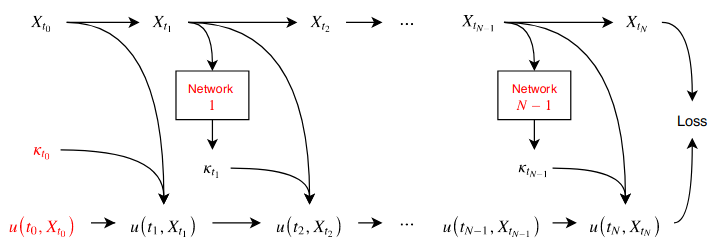
\includegraphics[width=\linewidth]{images/DeepBSDEMap}
	\caption{Deep BSDE diagram \cite{chan-wai-nam_machine_2018}. In red are the parameters to be optimized in the algorithm \hlc[Hay que cambiar $\kappa_i$]{}}
	\label{fig:deepbsdemap}
\end{figure}

The convergence of this algorithm has been proved in \cite{han_convergence_2020} for fully coupled FBSDEs. The assumptions needed are very general, and the proof is rather technical, so for the sake of brevity, we only state some imprecise results.

Denote by $X_t,Y_t,Z_t$ the exact solution to the FBSDE \eqref{eqn:UncoupledCh2}, and by $X_{t_i}^\pi,Y_{t_i}^\pi,Y_{t_i}^\pi$ the discrete solution to the constrained optimization problem \eqref{eqn:constrainedDeepBSDE}. Also, let's denote $h=\max_{i}\Delta t_i$. The first result states that the simulation error can be bounded through the value of the loss function \eqref{eqn:lossDeepBSDE}.
\begin{theorem}[Error of discretization is bounded by loss function \cite{han_convergence_2020}]
	Under some assumptions, there exist a constant $C$, independent of $h$, $d$ and $n$, such that for sufficiently small $h$
	$$
	\sup _{t \in[0, T]}\left(E\left|X_t-\hat{X}_t^\pi\right|^2+E\left|Y_t-\hat{Y}_t^\pi\right|^2\right)+\int_0^T E\left|Z_t-\hat{Z}_t^\pi\right|^2 \mathrm{~d} t \leq C\left[h+E\left|g\left(X_T^\pi\right)-Y_T^\pi\right|^2\right]
	$$
	where $\hat{X}_t^\pi=X_{t_i}^\pi, \hat{Y}_t^\pi=Y_{t_i}^\pi, \hat{Z}_t^\pi=Z_{t_i}^\pi$ for $t \in\left[t_i, t_{i+1}\right)$
\end{theorem}   

The second result establishes that the optimal value of the loss function can be small if the approximation capability of the family of parametric functions (neural networks) is good enough. Denote by $\mathcal{N}_0'$ and $\{\mathcal{N}_i\}_{0}^{N-1}$ the parametric function spaces generated by neural networks, then we have
\begin{theorem}[Optimal loss function is bounded by approximation error \cite{han_convergence_2020}]
Under some assumptions, there exists a constant $C$, independent of $\Delta t, d$ and $n$, such that for sufficiently small $\Delta t$,
	$$
	\begin{aligned}
		& \inf _{\mu_0^\pi \in \mathcal{N}_0^{\prime}, \phi_i^\pi \in \mathcal{N}_i} E\left|g\left(X_T^\pi\right)-Y_T^\pi\right|^2 \\
		& \leq C\left\{h+\inf _{\mu_0^\pi \in \mathcal{N}_0^{\prime}, \phi_i^\pi \in \mathcal{N}_i}\left[E\left|Y_0-\mu_0^\pi(\xi)\right|^2\right.\right. \\
		&\left.\left.+\sum_{i=0}^{N-1} E\left|E\left[\tilde{Z}_{t_i} \mid X_{t_i}^\pi, Y_{t_i}^\pi\right]-\phi_i^\pi\left(X_{t_i}^\pi, Y_{t_i}^\pi\right)\right|^2 h\right]\right\},
	\end{aligned}
	$$
	where $\tilde{Z}_{t_i}=h^{-1} E\left[\int_{t_i}^{t_{i+1}} Z_t \mathrm{~d} t \mid \mathcal{F}_{t_i}\right]$. If $\mu$ and $\sigma$ are independent of $Y$, the term $E\left[\tilde{Z}_{t_i} \mid X_{t_i}^\pi, Y_{t_i}^\pi\right]$ can be replaced with $E\left[\tilde{Z}_{t_i} \mid X_{t_i}^\pi\right]$.
\end{theorem}

Neural networks are a promising candidate for such approximation space of functions, as there are results in regard
to the universal approximation and complexity of neural networks\hlc[Completar referencias]{}.

Note that, in practice, we cannot minimize exactly the loss function in the space of parametric functions, as the methods we use are generally iterative. Also, it is not known how better is the approximation depending on the width, deep and connections of the neural network, so the capability of approximation is not well understood yet. Therefore, this results only establish the convergence of the method in a general setting and are not useful for estimate the real velocity of convergence, the achievable loss in the training stage, nor the real accuracy of the approximate solution.  

Now, we highlight the major drawbacks of this method 
\begin{enumerate}
	\item The number of neural networks to train grows linearly with the number of time steps in the discretization, making it very computationally costly to use small time steps.
	\item We only have a full solution at time $t=0$. At intermediate times we only have approximate solutions evaluated on sample paths $v(t,X_t)$. Therefore, we would need many of them to represent accurately the solution in the desired region.
	\item Moreover, nothing guarantees that this intermediate steps resembles accurately the real solutions in between steps. This requirement is not well encoded in the loss function.
	\item The time structure of the problem is not reflected in the separate approximations for each step, at least not directly.
	\item It may be unstable or converge to saddle points, see \cite{hure_deep_2020}.
\end{enumerate}     

Moreover, the structure of the neural networks is crucial for the practical convergence of the algorithm. The original work by \cite{han_solving_2018} used fully coupled neural networks with 3 layers, the $relu$ activation function and batch normalization. However, many changes can be made to accelerate the process of training or to achieve lower optimal losses. All of them are inspired by practical evidence and currently there is not enough understanding of how to choose theoretically the hyperparameters to reach the best convergence we can. Some of these modifications are explained below.


\subsubsection*{Merged Deep BSDE}
\subsubsection*{Residual Merged Deep BSDE}

\subsection{Raissi's method}
%\subsection{Deep Splitting/Tensor train?}
\subsection{An example}
\section{Boundary problems}
\subsection{Deep Galerkin method}
\subsection{Interpolating BSDEs with PINNs}
\subsection{Reflection on Boundary}

\subsection{An example with optimal control}